\subsection{Diseño Orientado a Objetos}

\subsubsection{Ciclo de vida de una consulta}

El siguiente diagrama (figura \ref{fig:sequence_sinatra}) muestra la interacción en los distintos componentes de la aplicaciones. Los distintos componentes serán explicados en las sucesivas secciones.

\begin{figure}[h]
\centerline{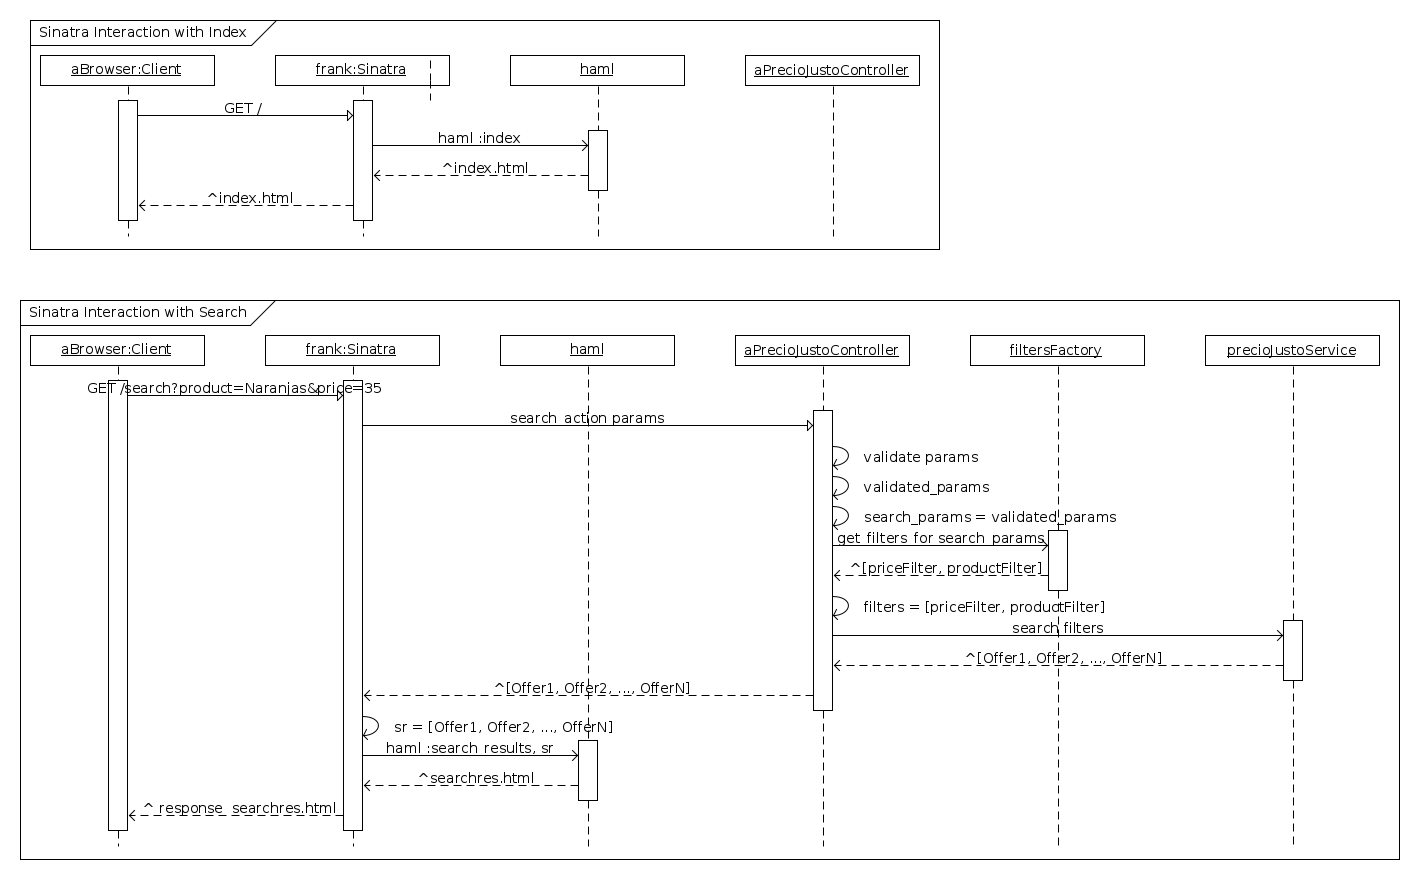
\includegraphics[width=0.9\paperwidth]{./imgs/sequence_diagram_sinatra.png}}
\caption{Diagrama de secuencia de sinatra}
\label{fig:sequence_sinatra}
\end{figure}


\subsubsection{Factory de servicios}
Dado que twitter permite dos tipos de obtención de tweets, vía streaming o por búsquedas, es que implementamos dos formas de trabajar con los tweets, pero que desde el lado de clientes de la búqueda de ofertas de El Precio de Justo mantienen la misma interfaz.

Para esto último decidimos utlizar el patrón de \texttt{abstract factory} con dos
implementaciones, una online y otra offline. Cada una de estas implementaciones nos permiten crear la clase de servicio apropiada (la clase que encapsula la lógica de la aplicación), los filtros permitidos y la implementación específica de estos.

Esto puede verse en la figura \ref{fig:class_service_factory}.

\begin{figure}[h]
\centerline{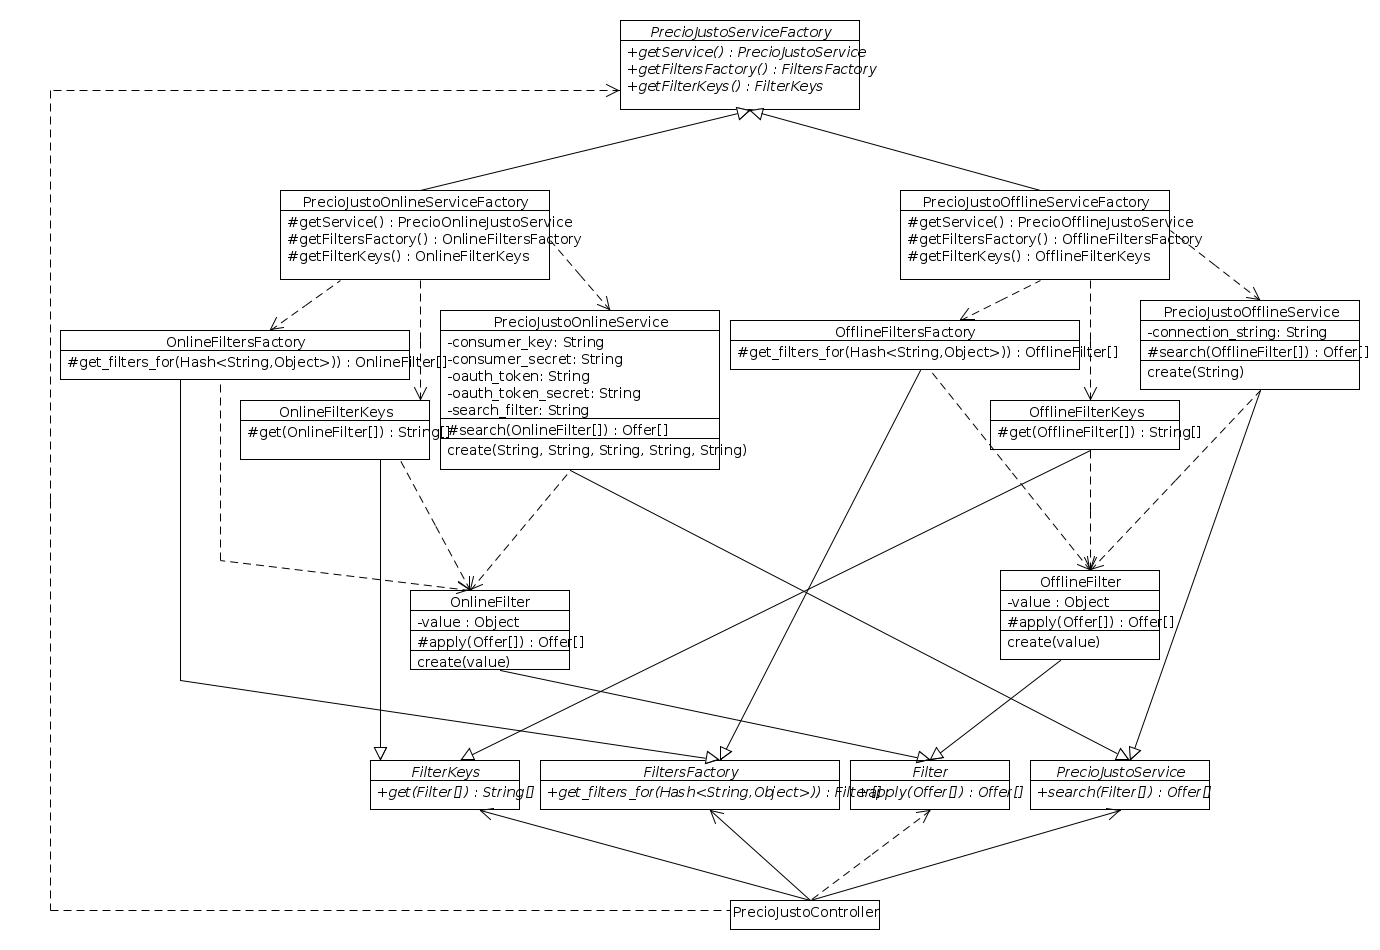
\includegraphics[width=0.9\paperwidth]{./imgs/class_diagram_service_factory_v2.png}}
\caption{Diagrama de clases de creación de servicios}
\label{fig:class_service_factory} 
\end{figure}

\subsubsection{Filtros}

Dado que el filtrado de los tweets de las ofertas búscadas se realizan de distinta manera, los filtros si bien deberán proveer las misma funcionalidad son implementativamente distintos.

En un caso filtrarán las ofertas que se vayan obtienendo de twitter en vivo y en el otro caso se realizará un búsqueda sobre el motor de base de datos.

Los filtros modelados son por porducto, precio y ubicación, si bien es posible extenderlos.

Esto puede verse en el diagrama de la figura \ref{fig:class_filter_factory}. 

\begin{figure}[h]
\centerline{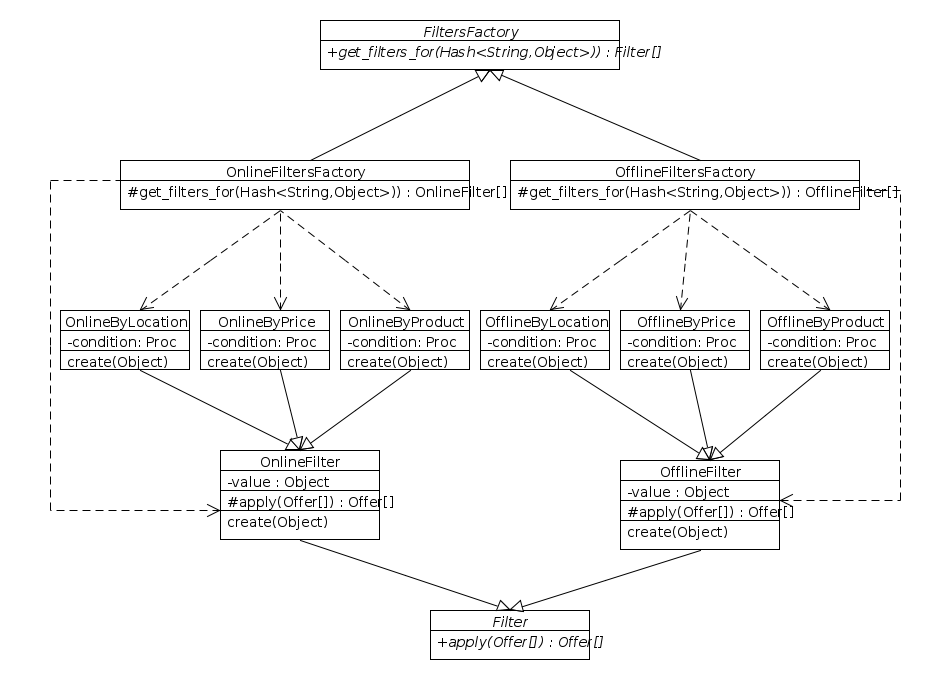
\includegraphics[width=\textwidth]{./imgs/class_diagram_filters_factory.png}}
\caption{Diagrama de clases de creación de filtros}
\label{fig:class_filter_factory} 
\end{figure}

\subsubsection{Extracción de datos de un tweet}
La extracción de las información de las ofertas que se encuentra en los tweets se realizar mediante objetos de la clase \texttt{OfferFromTweetExtractor} (clase abstracta).
Para la demostración realizamos una implementación que extrae la información mediante expresiones regulares para cada pedazo de información dentro del texto, salvo para la geolocalización del tweet.
Si bien no está implementado para la demo, es deseable delegar la creación de las instancias de Offer. Para ello pensamos realizar mediante un \texttt{OfferBuilder}, la tarea del mismo sería realizar las acciones necesarias para crear una nueva instanacia.

La idea es que cada pedazo de información genere una instancia de un objeto polimórfico de la información que modela (ej: el precio, producto, unidad).
Cuando nos referímos a objetos polimórficos, queremos decir que la información podría no poder generar un objeto válido y queremos que resulte transparente para los objetos con los que interactuan con dicho objeto (la idea es poder implementar \texttt{Null Object Pattern})

\begin{figure}[h]
\centerline{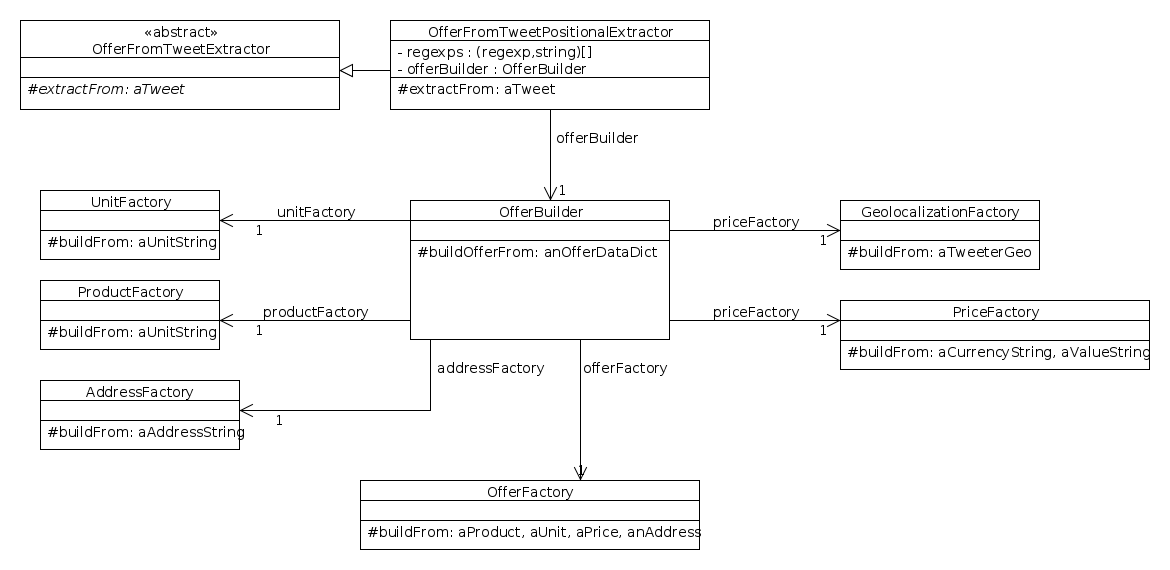
\includegraphics[width=\textwidth]{./imgs/class_diagram_parsing.png}}
\caption{Diagrama de clases de extraccion datos de tweet}
\label{fig:class_parsing}
\end{figure}

\begin{figure}[h]
\centerline{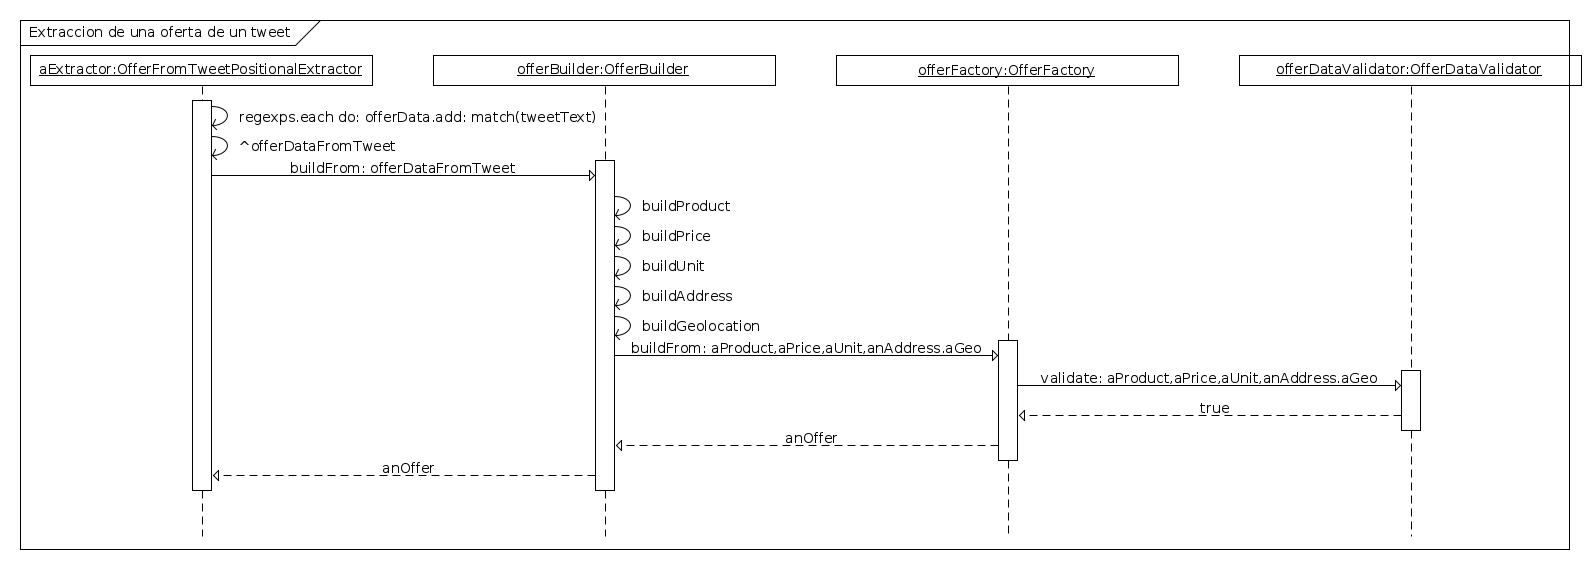
\includegraphics[width=\textwidth]{./imgs/sequence_diagram_parsing.png}}
\caption{Diagrama de secuencia de extraccion de datos de tweet}
\label{fig:secuence_parsing}
\end{figure}

\subsubsection{Servicio Online}
En este caso la clase PrecioJustoOnlineService encapsula la lógica de la aplicación utilizando como fuente de información las búsquedas directas en \texttt{Twitter} mediante la \texttt{API} de \texttt{Search}.
Para aplicar los filtros utiliza las clases derivadas de \texttt{OnlineFilter} y utiliza \texttt{OfferFromTweetPositionalExtractor} para la extracción de las ofertas.

\begin{figure}[h]
\centerline{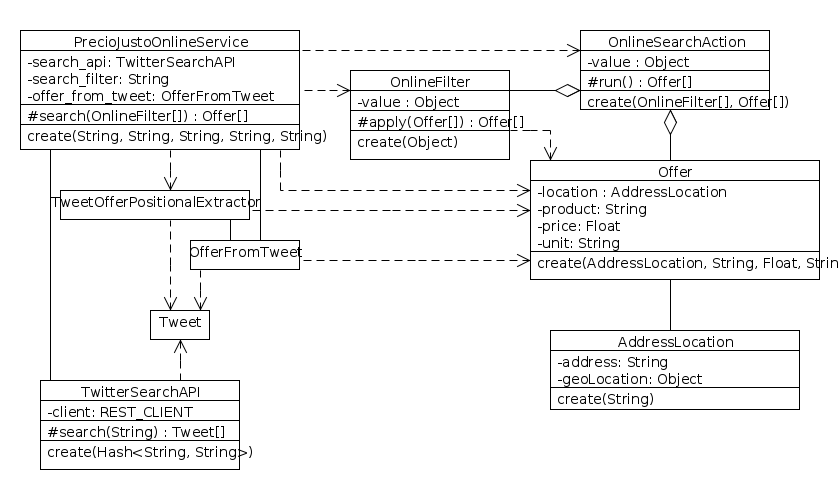
\includegraphics[width=\textwidth]{./imgs/class_diagram_online_service.png}}
\caption{Diagrama de clases de servicio online}
\label{fig:class_online_service}
\end{figure}

\subsubsection{Servicio Offline}

\textbf{PrecioJustoOfflineService}\\

En este caso la clase \texttt{PrecioJustoOfflineService} encapsula la lógica de la aplicación utilizando como fuente de información una base de datos \texttt{SQLite3}. La cual es alimentada mediante un servicio independiente.
Para aplicar los filtros utiliza las clases derivadas de \texttt{OfflineFilter}. Las ofertas
ya fueron parseadas antes de ser insertadas en la base de datos.

\begin{figure}[h]
\centerline{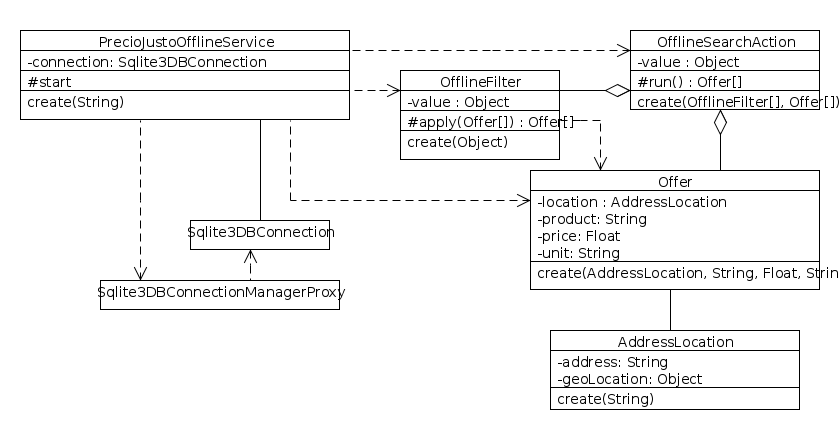
\includegraphics[width=\textwidth]{./imgs/class_diagram_offline_service.png}}
\caption{Diagrama de clases de servicio offline}
\label{fig:class_offline_service}
\end{figure}

\textbf{Servicio de Streaming}\\

Este proceso independiente utiliza la \texttt{API} de \texttt{Streaming} de \texttt{Twitter} para obtener las ofertas y persistirlas en la base de datos.
Para la extracción de las ofertas de los tweets utiliza el extractor \texttt{OfferFromTweetPositionalExtractor}.

\begin{figure}[h]
\centerline{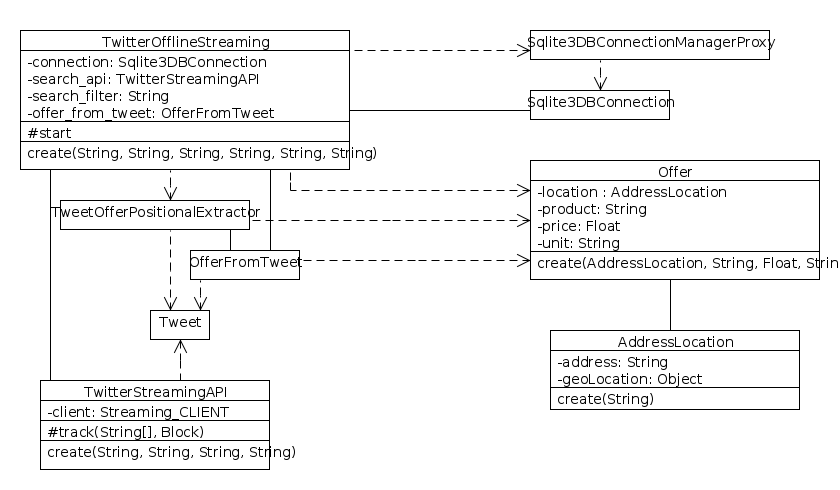
\includegraphics[width=\textwidth]{./imgs/class_diagram_offline_streaming.png}}
\caption{Diagrama de clases de streaming de twitter}
\label{fig:class_offline_streaming}
\end{figure}


\textbf{Cliente/Servidor SQLite3}\\

Dado la base de datos \texttt{SQLite3} es un archivo, el mismo se bloquea al accederlo
directamente. Para evitar esto generamos un proceso independiente que es el único que bloque el archivo, pero expone mediante \texttt{DRB (remoting)} la conexión a esta base para poder ser usada concurrentemente por distintos proceso.

\begin{figure}[h]
\centerline{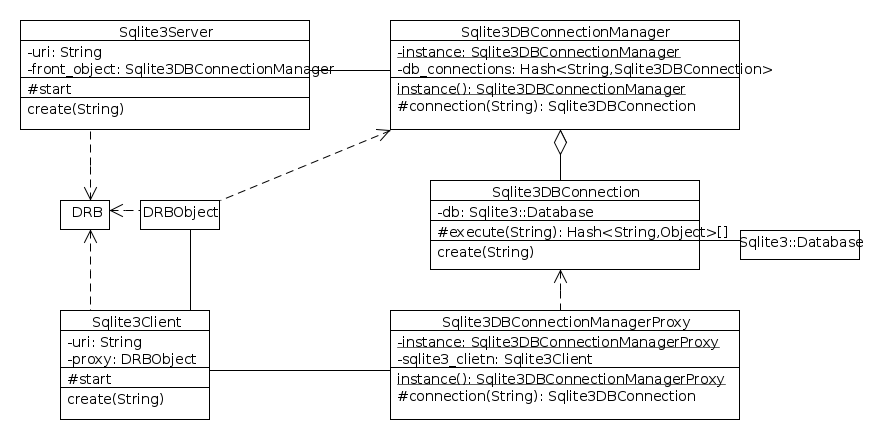
\includegraphics[width=\textwidth]{./imgs/class_diagram_sqlite3_client_server.png}}
\caption{Diagrama de clases de BD SQLite3}
\label{fig:class_sqlite3_client_server}
\end{figure}

\textbf{Ofertas y colaboradores}

El siguiente diagramas muestra el modelo de las ofertas (\texttt{Offer}) y sus colaboradores. Dichos colaboradores no están modelados en la demostración.
El siguiente diagramas muestra la idea de creación de los distintos objetos
con la idea de poder generar objetos no válidos polimórficos a los válidos.

\begin{figure}[h]
\centerline{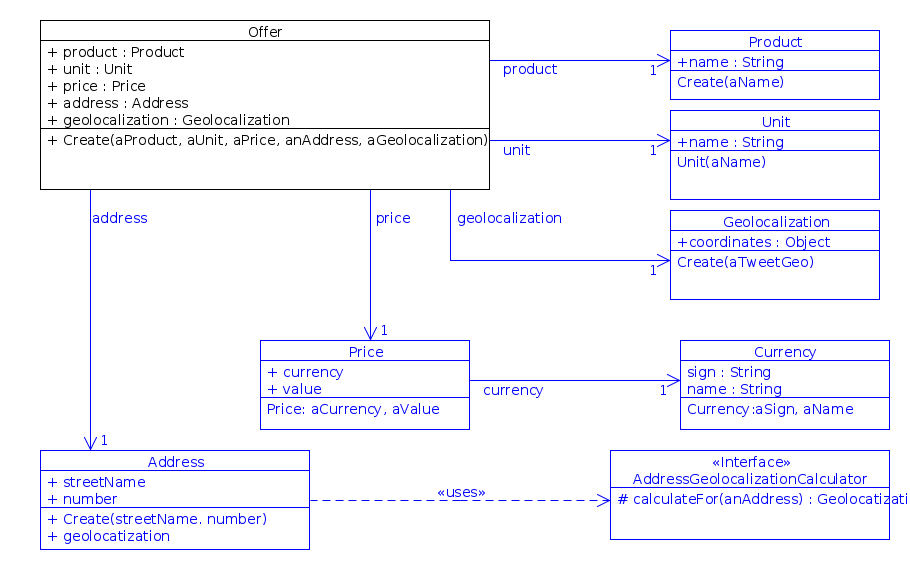
\includegraphics[width=\textwidth]{./imgs/class_diagram_offer.png}}
\caption{Diagrama de clases de offer y colaboradores}
\label{fig:class_offer}
\end{figure}

\begin{figure}[h]
\centerline{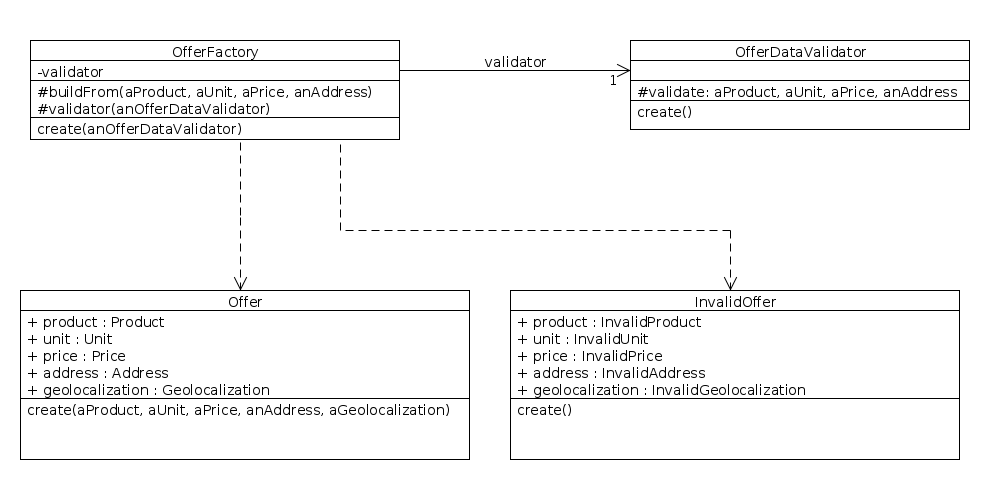
\includegraphics[width=\textwidth]{./imgs/class_diagram_Offer_Factory.png}}
\caption{Diagrama de clases de creación de offer}
\label{fig:class_Offer_Factory}
\end{figure}

